\section{Einleitung}

\begin{frame}[c]
	\frametitle{Brute-Force-Angriff auf klassische Verfahren}

	\begin{align*}
		K_1 &\rightarrow \text{yxV\#U}\\
		K_2 &\rightarrow \text{Katze}\\
		K_3 &\rightarrow \text{-CPK9}\\
		\dots &\rightarrow \dots
	\end{align*}

\end{frame}

\begin{frame}[c]
	\frametitle{Verwendete Passwörter}

	\begin{center}
		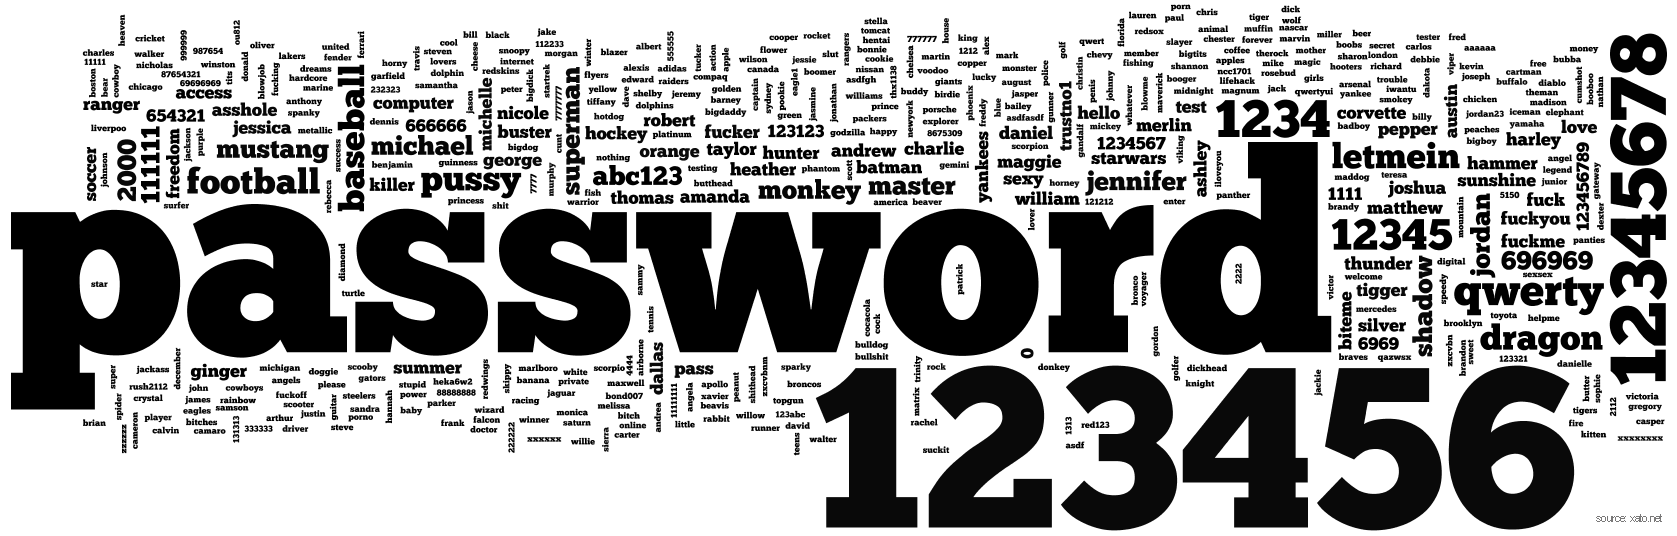
\includegraphics[width=\textwidth]{pic/passwordscloud.png}
		\vspace*{.5cm}
	\end{center}
	\hfill \tiny{\emph{https://xato.net/wp-content/xup/passwordscloud.png}}
\end{frame}

\begin{frame}[c]
	\frametitle{Honey Encryption - Idee}

	\begin{align*}
		K_1 &\rightarrow \text{Hund}\\
		K_2 &\rightarrow \text{Katze}\\
		K_3 &\rightarrow \text{Maus}\\
		\dots &\rightarrow \dots
	\end{align*}
	
\end{frame}

\begin{frame}[c]
	\frametitle{Honey Encryption}

	\begin{quote}
		Honey Encryption wurde entwickelt, um Ciphertexte zu generieren, die bei Entschlüsselung mit einem falschen Schlüssel zu einem plausibel wirkenden, aber unechten Klartext führen.
	\end{quote}
	
	\vspace*{1cm}

	\hfill \textit{- A. Juels, T. Ristenpart}
\end{frame}